% What was found and tested: the evidence behind the captioned music model (architecture.tex, the first sheet), in the
% same style. Colours: teal = what the model uses / our models; grey = the alternatives they were compared with; pink =
% captions. Sections are numbered in reading order.
% Sources: head-to-head from results/head2head/scores.{md,json}, scores_96*, bootstrap_*, midicaps/, text/clamp3.* (copies
% in docs/head2head/; eval/compare/head2head.py, h2h_midicaps.py, h2h_clamp3.py, adapters in eval/compare/h2h_baselines/,
% weights in checkpoints/baselines/); F1 run from logs/f1/f1_evals.log (f1-results Hub
% repo); caption phase from results/f1_post/ (steps.log, opening_gain.txt, text_eval/summary.md,
% length_follow/summary.md); decoding search from results/gen_search/f1/summary.md; style hold from
% config/generate/f1.toml; section recipe from config/pilots/section_*.py + logs/sections/forget.md; GQA from
% logs/sections/ + context/claude/caption_450m_2026-10-25.md; base run from config/pretrain/long_450m.py; fine-tune from
% config/finetune/finetune_ua450{,_multi}.py; song counts from data/finetune/ukrainian_{multi_v1,reduction_v4}.csv;
% audio pipeline from data_prep/songs/audio_to_piano.py; curves from curves/*.dat (python docs/figures/curves_data.py).
% Build: pdflatex findings.tex  (TinyTeX: export PATH=$HOME/.local/bin:$PATH; needs colortbl, mathastext, pgfplots)
% SVG / PNG: pdftocairo -svg findings.pdf findings.svg ; pdftocairo -png -r 200 -singlefile findings.pdf findings
\documentclass[border=8pt]{standalone}
\usepackage[T1]{fontenc}
\usepackage[scaled=0.92]{helvet}
\renewcommand{\familydefault}{\sfdefault}
\usepackage{inconsolata}
\usepackage{amsmath}
\usepackage[italic]{mathastext}     % maths letters and digits in Helvetica, like the text
\usepackage[table]{xcolor}
\usepackage{array}
\usepackage{tabularx}
\usepackage{pgfplots}
\pgfplotsset{compat=1.18}
\usepackage{tikz}
\usetikzlibrary{arrows.meta,calc,decorations.pathreplacing,backgrounds}
\usepackage[hidelinks]{hyperref}
\hyphenpenalty=10000
\exhyphenpenalty=10000

\definecolor{tealT}{HTML}{3B7D70}   % title, section numbers, what the model uses
\definecolor{tealF}{HTML}{C3E0D6}   % table header, cooldown band
\definecolor{tealB}{HTML}{6FA696}
\definecolor{greyF}{HTML}{F2F2F2}   % text panels
\definecolor{greyB}{HTML}{8A8A8A}
\definecolor{rowG}{HTML}{F2F2F2}    % alternating table rows
\definecolor{pinkL}{HTML}{C2577A}   % captions
\definecolor{pinkF}{HTML}{F6CCD9}
\definecolor{altG}{HTML}{767676}    % the alternative a choice was compared with

\tikzset{
  box/.style={draw=black, fill=white, rounded corners=3pt, minimum height=5.6mm, inner sep=3pt, align=center,
              font=\footnotesize, line width=0.6pt},
  panel/.style={draw=greyB, fill=greyF, rounded corners=8pt, line width=1pt},
  ptitle/.style={font=\small\bfseries, anchor=south west, inner sep=2pt},
  arr/.style={-{Stealth[length=2.4mm]}, line width=0.9pt},
  ptext/.style={font=\footnotesize, text=black!90, align=left, inner sep=8pt},
  cell/.style={anchor=north west, font=\scriptsize, text=black!85, align=left, inner sep=10pt},
}
\newcommand{\rcite}[1]{{\scriptsize[#1]}}
\newcommand{\capt}[1]{\textcolor{pinkL}{``#1''}}
\newcommand{\badge}[1]{\tikz[baseline=(b.base)]\node[circle, fill=tealT, text=white, inner sep=0pt, minimum size=4.4mm,
  font=\scriptsize\bfseries] (b) {#1};}
\newcommand{\sect}[2]{\badge{#1}\hspace{4pt}#2}
\newcommand{\hd}[1]{\textcolor{tealT}{\textbf{#1}}}
\newcommand{\us}[1]{\textcolor{tealT}{\textbf{#1}}}

\newlength{\panelW}
\setlength{\panelW}{\dimexpr 16.8cm + 9.2cm + 18pt\relax}
\begin{document}
%% ================= small drawings inside text panels =================
\newsavebox{\spliceBox}
\sbox{\spliceBox}{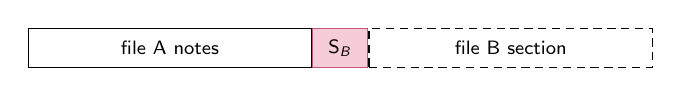
\begin{tikzpicture}
  \node[draw=black, fill=white, minimum width=36mm, minimum height=5mm, font=\scriptsize] (sa) at (0, 0) {file A notes};
  \node[draw=pinkL, fill=pinkF, minimum width=7mm, minimum height=5mm, font=\scriptsize, anchor=west] (sb) at (sa.east) {S$_B$};
  \node[draw=black, fill=white, minimum width=36mm, minimum height=5mm, font=\scriptsize, anchor=west, densely dashed] at (sb.east) {file B section};
\end{tikzpicture}}%

\newsavebox{\repeatBox}
\sbox{\repeatBox}{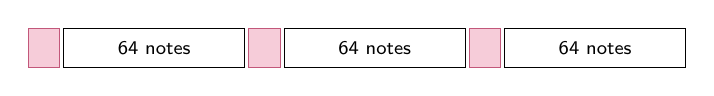
\begin{tikzpicture}
  \foreach \i in {0,1,2} {
    \node[draw=pinkL, fill=pinkF, minimum width=4mm, minimum height=5mm, inner sep=0pt] at (2.8*\i, 0) {};
    \node[draw=black, fill=white, minimum width=23mm, minimum height=5mm, font=\scriptsize] at (1.4+2.8*\i, 0) {64 notes};
  }
\end{tikzpicture}}%

%% ================= charts (pgfplots) =================
\pgfplotsset{cplot/.style={scale only axis, width=5.3cm, height=3.3cm, axis lines*=left, axis line style={black!55},
  tick style={black!55}, grid=major, grid style={black!10}, tick label style={font=\scriptsize}, label style={font=\scriptsize},
  every axis plot/.append style={line join=round}, clip=false, xlabel shift=-2pt, ylabel shift=-3pt,
  scaled ticks=false, tick label style={/pgf/number format/fixed}}}
\pgfplotsset{dots/.style={cplot, ymin=-0.6, y dir=reverse, grid=none, xmajorgrids, axis y line*=none,
  y axis line style={draw=none}, ytick style={draw=none}, yticklabel style={align=right, xshift=-6pt}}}

% head-to-head: D of each system's continuations (rows of curves/h2h_cont.dat: real, ours x 2, other models x 5;
% filled = the first 1,000 new notes, hollow = the first 200; Moonbeam at T 0.6 is off the scale at 1,000)
\newsavebox{\curveHH}
\sbox{\curveHH}{\begin{tikzpicture}
\begin{axis}[dots, width=4.6cm, height=5.6cm, ymax=7.6, xmin=0, xmax=0.75, xtick={0,0.2,0.4,0.6}, ytick={0,...,7},
    xlabel={D: distance to the real continuations (lower = closer)},
    yticklabels={{real continuation}, {musicar-L (464M)}, {musicar-L-caption (477M)}, {AMT large (780M)},
                 {SkyTNT medium (234M)}, {Music-Llama, SkyTNT\\architecture (457M)}, {Moonbeam, $T$ 0.9 (839M)},
                 {Moonbeam, $T$ 0.6 (839M)}}]
  \draw[black!25, line width=1.2pt] (axis cs:0, 1) -- (axis cs:0.121, 1);
  \node[anchor=west, font=\scriptsize, text=black!80, inner sep=4pt] at (axis cs:0.121, 1) {0.121};
  \draw[black!25, line width=1.2pt] (axis cs:0, 2) -- (axis cs:0.218, 2);
  \node[anchor=west, font=\scriptsize, text=black!80, inner sep=4pt] at (axis cs:0.218, 2) {0.218};
  \draw[black!25, line width=1.2pt] (axis cs:0, 3) -- (axis cs:0.289, 3);
  \node[anchor=west, font=\scriptsize, text=black!80, inner sep=4pt] at (axis cs:0.289, 3) {0.289};
  \draw[black!25, line width=1.2pt] (axis cs:0, 4) -- (axis cs:0.314, 4);
  \node[anchor=west, font=\scriptsize, text=black!80, inner sep=4pt] at (axis cs:0.314, 4) {0.314};
  \draw[black!25, line width=1.2pt] (axis cs:0, 5) -- (axis cs:0.357, 5);
  \node[anchor=west, font=\scriptsize, text=black!80, inner sep=4pt] at (axis cs:0.357, 5) {0.357};
    \draw[black!25, line width=1.2pt] (axis cs:0, 6) -- (axis cs:0.703, 6);
  \node[anchor=south east, font=\scriptsize, text=black!80, inner sep=3pt] at (axis cs:0.703, 6) {0.703};
  \draw[black!25, line width=1.2pt, -{Stealth[length=4pt]}] (axis cs:0, 7) -- (axis cs:0.75, 7);
  \node[anchor=south east, font=\scriptsize, text=black!80, inner sep=3pt] at (axis cs:0.75, 7) {1.316 $\rightarrow$};
  \node[anchor=west, font=\scriptsize, text=black!80, inner sep=4pt] at (axis cs:0, 0) {0 (the reference)};
  \addplot[black, only marks, mark=*, mark size=2.4pt] table[x=D, y expr=\coordindex, skip coords between index={1}{8}] {curves/h2h_cont.dat};
  \addplot[tealT, only marks, mark=*, mark size=2.8pt] table[x=D, y expr=\coordindex, skip coords between index={0}{1}, skip coords between index={3}{8}] {curves/h2h_cont.dat};
  \addplot[altG, only marks, mark=*, mark size=2.4pt] table[x=D, y expr=\coordindex, skip coords between index={0}{3}, skip coords between index={7}{8}] {curves/h2h_cont.dat};
  \addplot[tealT, only marks, mark=o, mark size=2.8pt, line width=1pt, fill=white] table[x=D200, y expr=\coordindex, skip coords between index={0}{1}, skip coords between index={3}{8}] {curves/h2h_cont.dat};
  \addplot[altG, only marks, mark=o, mark size=2.4pt, line width=1pt, fill=white] table[x=D200, y expr=\coordindex, skip coords between index={0}{3}] {curves/h2h_cont.dat};
\end{axis}
\end{tikzpicture}}%

\newsavebox{\hhTable}
\sbox{\hhTable}{\scriptsize\renewcommand{\arraystretch}{1.3}\setlength{\tabcolsep}{4.5pt}%
\begin{tabular}{@{}lrrrrrrrrrrr@{}}
system & notes / s & instr. & out of band & top share & takeover & runaway & copies & ended & D & D, 200 & params\\\hline
real continuation & 24.0 & 7.69 & 0.153 & 0.390 & 0 & 0.156 & 0.049 & 0.22 & 0 & 0 & \\
\us{musicar-L} & 23.5 & 6.91 & 0.103 & 0.418 & 0 & 0.125 & 0.144 & 0.31 & \textbf{0.121} & \textbf{0.090} & 464M\\
\us{musicar-L-caption} & 12.8 & 7.78 & 0.170 & 0.415 & 0 & 0.063 & 0 & 0.53 & \textbf{0.218} & 0.198 & 477M\\
AMT large \rcite{15} & 21.2 & 7.44 & 0.117 & 0.468 & 0.094 & 0.063 & 0.043 & 0.78 & 0.289 & 0.239 & 780M\\
SkyTNT medium \rcite{16} & 22.9 & 5.34 & 0 & 0.439 & 0.031 & 0.156 & 0.136 & 0.28 & 0.314 & 0.184 & 234M\\
Music-Llama \rcite{17} & 28.9 & 5.69 & 0.020 & 0.439 & 0.031 & 0.250 & 0.137 & 0.25 & 0.357 & 0.218 & 457M\\
Moonbeam \rcite{21}, $T$ 0.9 & 49.5 & 8.88 & 0.140 & 0.491 & 0.156 & 0.312 & 0.208 & 0.16 & 0.703 & 0.322 & 839M\\
Moonbeam, $T$ 0.6 & 85.9 & 5.25 & 0.018 & 0.533 & 0.125 & 0.063 & 0.456 & 0 & 1.316 & 0.525 & 839M\\
\end{tabular}}%

\newsavebox{\curveHHp}
\sbox{\curveHHp}{\begin{tikzpicture}
\begin{axis}[dots, width=4.3cm, height=3.6cm, ymax=4.6, xmin=0, xmax=0.2, xtick={0,0.05,0.1,0.15,0.2}, ytick={0,...,4},
    xlabel={D: distance to the real continuations (lower = closer)},
    yticklabels={{real continuation}, {108M piano covers (ua\_2048\_v2)}, {musicar-L (464M)}, {Aria medium (659M)},
                 {450M piano-cover fine-tune}}]
  \draw[black!25, line width=1.2pt] (axis cs:0, 1) -- (axis cs:0.018, 1);
  \node[anchor=west, font=\scriptsize, text=black!80, inner sep=4pt] at (axis cs:0.018, 1) {0.018};
  \draw[black!25, line width=1.2pt] (axis cs:0, 2) -- (axis cs:0.040, 2);
  \node[anchor=west, font=\scriptsize, text=black!80, inner sep=4pt] at (axis cs:0.040, 2) {0.040};
  \draw[black!25, line width=1.2pt] (axis cs:0, 3) -- (axis cs:0.096, 3);
  \node[anchor=west, font=\scriptsize, text=black!80, inner sep=4pt] at (axis cs:0.096, 3) {0.096};
  \draw[black!25, line width=1.2pt] (axis cs:0, 4) -- (axis cs:0.177, 4);
  \node[anchor=west, font=\scriptsize, text=black!80, inner sep=4pt] at (axis cs:0.177, 4) {0.177};
  \node[anchor=west, font=\scriptsize, text=black!80, inner sep=4pt] at (axis cs:0, 0) {0 (the reference)};
  \addplot[black, only marks, mark=*, mark size=2.4pt] table[x=D, y expr=\coordindex, skip coords between index={1}{5}] {curves/h2h_piano.dat};
  \addplot[tealT, only marks, mark=*, mark size=2.8pt] table[x=D, y expr=\coordindex, skip coords between index={0}{1}, skip coords between index={3}{4}] {curves/h2h_piano.dat};
  \addplot[altG, only marks, mark=*, mark size=2.4pt] table[x=D, y expr=\coordindex, skip coords between index={0}{3}, skip coords between index={4}{5}] {curves/h2h_piano.dat};
  \addplot[tealT, only marks, mark=o, mark size=2.8pt, line width=1pt, fill=white] table[x=D200, y expr=\coordindex, skip coords between index={0}{1}, skip coords between index={3}{4}] {curves/h2h_piano.dat};
  \addplot[altG, only marks, mark=o, mark size=2.4pt, line width=1pt, fill=white] table[x=D200, y expr=\coordindex, skip coords between index={0}{3}, skip coords between index={4}{5}] {curves/h2h_piano.dat};
\end{axis}
\end{tikzpicture}}%

\newsavebox{\hhPiano}
\sbox{\hhPiano}{\scriptsize\renewcommand{\arraystretch}{1.3}\setlength{\tabcolsep}{4.5pt}%
\begin{tabular}{@{}lrrrrrrrr@{}}
system & notes / s & runaway & ended & copies & prompt check & D & D, 200 & params\\\hline
real continuation & 7.95 & 0 & 0 & 0.001 & 1 & 0 & 0 & \\
\us{108M piano covers} (ua\_2048\_v2, not released) & 8.39 & 0 & 0.34 & 0.001 & 1 & \textbf{0.018} & \textbf{0.006} & 108M\\
\us{musicar-L} & 8.95 & 0 & 0.41 & 0.003 & 1 & \textbf{0.040} & \textbf{0.019} & 464M\\
Aria medium, continuation \rcite{20} & 9.99 & 0.031 & 0.31 & 0.007 & 1 & 0.096 & 0.067 & 659M\\
\us{450M piano-cover fine-tune} (not released) & 3.53 & 0 & 1.00 & 0 & 1 & 0.177 & 0.078 & 464M\\
\end{tabular}}%

\newsavebox{\curveHHn}
\sbox{\curveHHn}{\begin{tikzpicture}
\begin{axis}[dots, width=4.6cm, height=4.0cm, ymax=5.6, xmin=0, xmax=0.62, xtick={0,0.2,0.4,0.6}, ytick={0,...,5},
    xlabel={D: distance to the real continuations (lower = closer)},
    yticklabels={{real continuation}, {musicar-L (464M)}, {musicar-L-caption (477M)}, {AMT large (780M)},
                 {SkyTNT medium (234M)}, {Music-Llama, SkyTNT\\architecture (457M)}}]
  \draw[black!25, line width=1.2pt] (axis cs:0, 1) -- (axis cs:0.144, 1);
  \node[anchor=west, font=\scriptsize, text=black!80, inner sep=4pt] at (axis cs:0.144, 1) {0.144};
  \draw[black!25, line width=1.2pt] (axis cs:0, 2) -- (axis cs:0.179, 2);
  \node[anchor=west, font=\scriptsize, text=black!80, inner sep=4pt] at (axis cs:0.205, 2) {0.179};
  \draw[black!25, line width=1.2pt] (axis cs:0, 3) -- (axis cs:0.097, 3);
  \node[anchor=west, font=\scriptsize, text=black!80, inner sep=4pt] at (axis cs:0.099, 3) {0.097};
  \draw[black!25, line width=1.2pt] (axis cs:0, 4) -- (axis cs:0.280, 4);
  \node[anchor=west, font=\scriptsize, text=black!80, inner sep=4pt] at (axis cs:0.280, 4) {0.280};
  \draw[black!25, line width=1.2pt] (axis cs:0, 5) -- (axis cs:0.561, 5);
  \node[anchor=south east, font=\scriptsize, text=black!80, inner sep=3pt] at (axis cs:0.561, 5) {0.561};
  \node[anchor=west, font=\scriptsize, text=black!80, inner sep=4pt] at (axis cs:0, 0) {0 (the reference)};
  \addplot[black, only marks, mark=*, mark size=2.4pt] table[x=D, y expr=\coordindex, skip coords between index={1}{6}] {curves/h2h_cont96.dat};
  \addplot[tealT, only marks, mark=*, mark size=2.8pt] table[x=D, y expr=\coordindex, skip coords between index={0}{1}, skip coords between index={3}{6}] {curves/h2h_cont96.dat};
  \addplot[altG, only marks, mark=*, mark size=2.4pt] table[x=D, y expr=\coordindex, skip coords between index={0}{3}] {curves/h2h_cont96.dat};
  \addplot[tealT, only marks, mark=o, mark size=2.8pt, line width=1pt, fill=white] table[x=D200, y expr=\coordindex, skip coords between index={0}{1}, skip coords between index={3}{6}] {curves/h2h_cont96.dat};
  \addplot[altG, only marks, mark=o, mark size=2.4pt, line width=1pt, fill=white] table[x=D200, y expr=\coordindex, skip coords between index={0}{3}] {curves/h2h_cont96.dat};
\end{axis}
\end{tikzpicture}}%

\newsavebox{\hhGroups}
\sbox{\hhGroups}{\scriptsize\renewcommand{\arraystretch}{1.3}\setlength{\tabcolsep}{4.5pt}%
\begin{tabular}{@{}lrrrrr@{}}
prompts & \us{musicar-L} & \us{musicar-L-caption} & AMT large & SkyTNT medium & Music-Llama\\\hline
all 96 & 0.144 & 0.179 & \textbf{0.097} & 0.280 & 0.561\\
\quad the published 32 & \textbf{0.121} & 0.218 & 0.289 & 0.314 & 0.357\\
\quad the new 64 & 0.181 & \textbf{0.159} & 0.224 & 0.295 & 0.693\\
\quad no-drums folder (65; most of these have drums) & 0.137 & 0.200 & \textbf{0.094} & 0.286 & 0.485\\
\quad with-drums folder (31) & 0.246 & \textbf{0.199} & 0.371 & 0.316 & 0.846\\
all 96, first 200 notes & \textbf{0.084} & 0.205 & 0.099 & 0.161 & 0.219\\
\quad the published 32 & \textbf{0.090} & 0.198 & 0.239 & 0.184 & 0.218\\
\quad the new 64 & 0.098 & 0.215 & \textbf{0.047} & 0.155 & 0.264\\
\end{tabular}}%

\newsavebox{\hhPianoN}
\sbox{\hhPianoN}{\scriptsize\renewcommand{\arraystretch}{1.3}\setlength{\tabcolsep}{4.5pt}%
\begin{tabular}{@{}lrrrrrr@{}}
piano, 96 prompts & notes / s & runaway & ended & D & D, 200 & closer than Aria\\\hline
real continuation & 8.31 & 0 & 0 & 0 & 0 & \\
\us{108M piano covers} (ua\_2048\_v2, not released) & 8.61 & 0 & 0.29 & \textbf{0.012} & \textbf{0.003} & 98\%\\
\us{musicar-L} & 9.19 & 0 & 0.48 & \textbf{0.035} & \textbf{0.016} & 93\%\\
Aria medium, continuation \rcite{20} & 9.93 & 0.021 & 0.20 & 0.074 & 0.044 & \\
\us{450M piano-cover fine-tune} (not released) & 3.75 & 0 & 0.91 & 0.182 & 0.081 & 0.1\%\\
\end{tabular}}%

\newsavebox{\curveHHt}
\sbox{\curveHHt}{\begin{tikzpicture}
\begin{axis}[dots, width=4.6cm, height=4.1cm, ymax=5.6, xmin=0, xmax=1.3, xtick={0,0.25,0.5,0.75,1,1.25}, ytick={0,...,5},
    xlabel={F: caption following (higher = follows)},
    yticklabels={{musicar-L-caption (477M)}, {musicar-L-caption,\\with \texttt{-{}-retrieve}}, {107M caption pilot s50\\(best of 4)},
                 {band fine-tune, caption\\picks + ranks (best of 4)}, {MIDI-LLM (1.72B)}, {Text2midi (250M)}}]
  \draw[black!25, line width=1.2pt] (axis cs:0.951, 0) -- (axis cs:1.073, 0);
  \draw[black!25, line width=1.2pt] (axis cs:1.08, 1) -- (axis cs:1.146, 1);
  \draw[black!25, line width=1.2pt] (axis cs:1.158, 2) -- (axis cs:1.164, 2);
  \draw[black!25, line width=1.2pt] (axis cs:1.123, 3) -- (axis cs:1.218, 3);
  \draw[black!25, line width=1.2pt] (axis cs:0.092, 4) -- (axis cs:0.604, 4);
  \draw[black!25, line width=1.2pt] (axis cs:0.06, 5) -- (axis cs:0.541, 5);
  \addplot[tealT, only marks, mark=*, mark size=2.8pt] table[x=F_en, y expr=\coordindex, skip coords between index={4}{6}] {curves/h2h_text.dat};
  \addplot[tealT, only marks, mark=o, mark size=2.8pt, line width=1pt, fill=white] table[x=F_uk, y expr=\coordindex, skip coords between index={4}{6}] {curves/h2h_text.dat};
  \addplot[altG, only marks, mark=*, mark size=2.4pt] table[x=F_en, y expr=\coordindex, skip coords between index={0}{4}] {curves/h2h_text.dat};
  \addplot[altG, only marks, mark=o, mark size=2.4pt, line width=1pt, fill=white] table[x=F_uk, y expr=\coordindex, skip coords between index={0}{4}] {curves/h2h_text.dat};
\end{axis}
\end{tikzpicture}}%

\newsavebox{\textTable}
\sbox{\textTable}{\scriptsize\renewcommand{\arraystretch}{1.3}\setlength{\tabcolsep}{4.5pt}%
\begin{tabular}{@{}lrrrrrrrrr@{}}
system & F, EN & F, UK & caption match & runaway & copies & notes / s & instr. & seconds & params\\\hline
\us{musicar-L-caption} (app preset, 60 s) & 1.07 & 0.95 & 0.857 & 0.021 & 0.031 & 8.8 & 9.5 & 63.5 & 477M\\
\us{musicar-L-caption} with \texttt{-{}-retrieve} (60 s) & \textbf{1.08} & \textbf{1.15} & \textbf{0.871} & 0.024 & 0.005 & 12.1 & 4.7 & 49.2 & 477M\\
\us{107M caption pilot s50} (best of 4) & 1.16 & 1.16 & 0.972 & 0.009 & 0.081 & 12.2 & 3.5 & 88.5 & 119M\\
\us{band fine-tune}, no text input (best of 4) & 1.12 & 1.22 & 0.981 & 0.011 & 0.068 & 15.1 & 3.4 & 61.0 & 464M\\
MIDI-LLM \rcite{18} & 0.60 & 0.09 & 0.553 & 0.141 & 0.021 & 24.6 & 3.0 & 35.0 & 1.72B\\
Text2midi \rcite{19} & 0.54 & 0.06 & 0.554 & 0.090 & 0.016 & 23.3 & 11.4 & 25.2 & 250M\\
\end{tabular}}%

\newsavebox{\curveHHm}
\sbox{\curveHHm}{\begin{tikzpicture}
\begin{axis}[dots, width=4.9cm, height=3.3cm, ymax=4.6, xmin=0, xmax=0.85, xtick={0,0.2,0.4,0.6,0.8}, ytick={0,...,4},
    xlabel={score (higher = closer to the caption)},
    yticklabels={{tempo bin (TB)}, {exact key (CK)}, {instrument recall}, {caption match (ours)}, {CLaMP 3 MRR}}]
  \draw[black!25, line width=1.2pt] (axis cs:0.248, 0) -- (axis cs:0.608, 0);
  \draw[black!25, line width=1.2pt] (axis cs:0.051, 1) -- (axis cs:0.586, 1);
  \draw[black!25, line width=1.2pt] (axis cs:0.167, 2) -- (axis cs:0.809, 2);
  \draw[black!25, line width=1.2pt] (axis cs:0.388, 3) -- (axis cs:0.711, 3);
  \draw[black!25, line width=1.2pt] (axis cs:0.052, 4) -- (axis cs:0.469, 4);
  \addplot[black, only marks, mark=|, mark size=3pt, line width=1pt] table[x=real, y expr=\coordindex] {curves/h2h_midicaps.dat};
  \addplot[black, only marks, mark=|, mark size=3pt, line width=1pt] table[x=real_shuffled, y expr=\coordindex] {curves/h2h_midicaps.dat};
  \addplot[tealT, only marks, mark=*, mark size=2.8pt] table[x=f1, y expr=\coordindex] {curves/h2h_midicaps.dat};
  \addplot[altG, only marks, mark=*, mark size=2.4pt] table[x=midi_llm, y expr=\coordindex] {curves/h2h_midicaps.dat};
  \addplot[altG, only marks, mark=o, mark size=2.4pt, line width=1pt] table[x=text2midi, y expr=\coordindex] {curves/h2h_midicaps.dat};
\end{axis}
\end{tikzpicture}}%

\newsavebox{\hhMidicaps}
\sbox{\hhMidicaps}{\scriptsize\renewcommand{\arraystretch}{1.3}\setlength{\tabcolsep}{4.5pt}%
\begin{tabular}{@{}lrrrrr@{}}
score & \us{musicar-L-caption} & MIDI-LLM \rcite{18} & Text2midi \rcite{19} & real files (ceiling) & shuffled (floor)\\\hline
TB: tempo in the asked bin & 0.244 & \textbf{0.400} & 0.345 & 0.608 & 0.248\\
TBT: or a neighbouring bin & 0.620 & \textbf{0.640} & \textbf{0.640} & 0.739 & 0.600\\
CK: exact key & 0.042 & \textbf{0.317} & 0.309 & 0.586 & 0.051\\
CKD: or the relative major / minor & 0.075 & \textbf{0.420} & 0.378 & 0.636 & 0.099\\
instrument recall & 0.425 & \textbf{0.664} & 0.426 & 0.809 & 0.167\\
family recall & 0.728 & \textbf{0.812} & 0.685 & 0.856 & 0.392\\
instrument Jaccard & 0.250 & \textbf{0.554} & 0.221 & 0.671 & 0.093\\
caption match (our thresholds) & 0.526 & \textbf{0.609} & 0.557 & 0.711 & 0.388\\
CLaMP 3 \rcite{22} MRR, caption finds its piece & 0.122 & \textbf{0.276} & 0.156 & 0.469 & 0.052\\
CLaMP 3 Fr\'echet to real files (lower = closer) & 193 & \textbf{112} & 154 & 33 & \\
seconds, notes / s in the first 40 s & 40.4, 13.6 & 28.8, 25.3 & 22.2, 22.4 & 37.9, 16.9 & \\
runaway (10-s windows) & \textbf{0.036} & 0.148 & 0.072 & 0.059 & \\
\end{tabular}}%

\newsavebox{\curveFone}
\sbox{\curveFone}{\begin{tikzpicture}
\begin{axis}[cplot, clip=true, clip mode=individual, xmin=0, xmax=2.1, ymin=1.72, ymax=1.98,
    xtick={0,0.5,1,1.5,2}, ytick={1.75,1.8,1.85,1.9,1.95}, xlabel={notes seen in F1 (billions)},
    ylabel={CE (nats / note)}]
  \fill[tealF!55] (axis cs:1.630, 1.72) rectangle (axis cs:2.1, 1.98);
  \node[anchor=north, font=\scriptsize, text=black!75, align=center] at (axis cs:1.865, 1.977) {WSD\\cooldown};
  \addplot[tealT, line width=1.6pt] table[x=notes, y=ce] {curves/f1_run.dat};
  \addplot[tealB, dashed, line width=1.3pt] table[x=notes, y=clean] {curves/f1_run.dat};
  \node[anchor=south west, font=\scriptsize, text=tealT] at (axis cs:0.25, 1.945) {held-out, captioned};
  \node[anchor=north west, font=\scriptsize, text=black!85] at (axis cs:0.25, 1.822) {clean GigaMIDI};
  \node[anchor=west, font=\scriptsize, text=tealT] at (axis cs:2.1, 1.882) {1.882};
  \node[anchor=west, font=\scriptsize, text=black!85] at (axis cs:2.1, 1.750) {1.750};
\end{axis}
\end{tikzpicture}}%

\newsavebox{\capTable}
\sbox{\capTable}{\scriptsize\renewcommand{\arraystretch}{1.3}\setlength{\tabcolsep}{5pt}%
\begin{tabular}{@{}lrr@{}}
 & F1 & \us{f1\_cap}\\\hline
held-out captioned CE (2,048 notes) & 1.882 & 1.898\\
clean GigaMIDI CE & 1.750 & 1.763\\
caption gain, notes 1--4 (vs none) & +0.377 & +0.348\\
caption gain, notes 1--32 (vs none) & +0.072 & +0.068\\
section gain (vs shuffled captions) & +0.0038 & +0.0058\\
text follow F, guidance 1 & 0.77 & 0.82\\
text follow F, guidance 2 & 0.82 & \textbf{1.03}\\
\quad EN / UK pairs at guidance 2 & 0.79 / 0.86 & 1.07 / 0.97\\
\end{tabular}}%

\newsavebox{\lenTable}
\sbox{\lenTable}{\scriptsize\renewcommand{\arraystretch}{1.3}\setlength{\tabcolsep}{5pt}%
\begin{tabular}{@{}lrrr@{}}
asked for & F1 & \us{f1\_cap} & f1\_cap, ramp 1$^*$\\\hline
nothing: median end & 142 s & 66 s & 68 s\\
30 s: end / asked, within 20\% & 1.09, 72\% & 1.04, 75\% & 1.07, 72\%\\
60 s & 1.01, 84\% & 0.96, 81\% & 1.00, 75\%\\
120 s & 0.91, 44\% & 0.97, 56\% & 0.98, \textbf{81\%}\\
\end{tabular}}%

\newsavebox{\curveBlock}
\sbox{\curveBlock}{\begin{tikzpicture}
\begin{axis}[cplot, xmin=250, xmax=1500, ymin=2.8, ymax=7.8, xtick={250,500,750,1000,1250,1500},
    xlabel={training step}, ylabel={val CE (nats / note)}]
  \foreach \s in {1,2,3} {
    \addplot[altG, dashed, line width=0.5pt] table {curves/block_base_s\s.dat};
    \addplot[tealT, line width=0.5pt] table {curves/block_newblock_s\s.dat};
  }
  \addplot[altG, dashed, line width=1.6pt] table {curves/block_base_mean.dat};
  \addplot[tealT, line width=1.6pt] table {curves/block_newblock_mean.dat};
  \node[anchor=west, font=\scriptsize, text=black!85, align=left] at (axis cs:1520, 3.95) {old 3.89};
  \node[anchor=west, font=\scriptsize, text=black!85, align=left] at (axis cs:1520, 3.08) {new 3.14};
\end{axis}
\end{tikzpicture}}%

\newsavebox{\curveBase}
\sbox{\curveBase}{\begin{tikzpicture}
\begin{axis}[cplot, xmin=0, xmax=8.3, ymin=1.6, ymax=2.9, xtick={0,2,4,6,8}, ytick={1.6,1.8,2.0,2.2,2.4,2.6,2.8},
    xlabel={notes seen (billions)}, ylabel={val CE (nats / note)}]
  \fill[tealF!55] (axis cs:6.636, 1.6) rectangle (axis cs:8.3, 2.9);
  \node[anchor=north, font=\scriptsize, text=black!75, align=center] at (axis cs:7.47, 2.88) {WSD\\cooldown};
  \addplot[tealT, line width=1.6pt] table[x=notes, y=ce] {curves/base_450m.dat};
  \fill[tealT] (axis cs:8.2956, 1.679) circle (2.2pt);
  \node[anchor=west, font=\scriptsize, text=black!85] at (axis cs:8.4, 1.679) {1.679};
  \node[anchor=south west, font=\scriptsize, text=black!85] at (axis cs:0.25, 2.807) {2.807 at 0.13B};
\end{axis}
\end{tikzpicture}}%

\newsavebox{\curveArms}
\sbox{\curveArms}{\begin{tikzpicture}
\pgfplotsset{arms/.style={cplot, width=2.5cm, height=4.6cm, ymin=-0.6, ymax=6.6, ytick={0,1,2,3,4,5,6}, grid=none,
    xmajorgrids, axis y line*=none, y axis line style={draw=none}, ytick style={draw=none},
    yticklabel style={align=right}}}
\begin{axis}[arms, name=sw, xmin=0, xmax=1.1, xtick={0,0.5,1}, xlabel={switch score (higher = follows)},
    yticklabels={{none (ctrl)}, {repeat}, {counterfactual}, {splice}, {all three}, {all three\\+ v2 words}, {splice 50\%,\\repeat, v2}}]
  \draw[black!25, line width=1.2pt] (axis cs:0, 0) -- (axis cs:0.06, 0);
  \node[anchor=west, font=\scriptsize, text=black!80, inner sep=1.5pt, xshift=2.5pt, fill=greyF] at (axis cs:0.06, 0) {0.06};
  \draw[black!25, line width=1.2pt] (axis cs:0, 1) -- (axis cs:0.09, 1);
  \node[anchor=west, font=\scriptsize, text=black!80, inner sep=1.5pt, xshift=2.5pt, fill=greyF] at (axis cs:0.09, 1) {0.09};
  \draw[black!25, line width=1.2pt] (axis cs:0, 2) -- (axis cs:0.13, 2);
  \node[anchor=west, font=\scriptsize, text=black!80, inner sep=1.5pt, xshift=2.5pt, fill=greyF] at (axis cs:0.13, 2) {0.13};
  \draw[black!25, line width=1.2pt] (axis cs:0, 3) -- (axis cs:0.59, 3);
  \node[anchor=west, font=\scriptsize, text=black!80, inner sep=1.5pt, xshift=2.5pt, fill=greyF] at (axis cs:0.59, 3) {0.59};
  \draw[black!25, line width=1.2pt] (axis cs:0, 4) -- (axis cs:0.85, 4);
  \node[anchor=west, font=\scriptsize, text=black!80, inner sep=1.5pt, xshift=2.5pt, fill=greyF] at (axis cs:0.85, 4) {0.85};
  \draw[black!25, line width=1.2pt] (axis cs:0, 5) -- (axis cs:0.94, 5);
  \node[anchor=west, font=\scriptsize, text=black!80, inner sep=1.5pt, xshift=2.5pt, fill=greyF] at (axis cs:0.94, 5) {0.94};
  \draw[black!25, line width=1.2pt] (axis cs:0, 6) -- (axis cs:0.98, 6);
  \node[anchor=west, font=\scriptsize, text=black!80, inner sep=1.5pt, xshift=2.5pt, fill=greyF] at (axis cs:0.98, 6) {0.98};
  \addplot[altG, only marks, mark=*, mark size=2.4pt] table[x=switch, y expr=\coordindex, skip coords between index={6}{7}] {curves/section_arms.dat};
  \addplot[tealT, only marks, mark=*, mark size=2.8pt] table[x=switch, y expr=\coordindex, skip coords between index={0}{6}] {curves/section_arms.dat};
\end{axis}
\begin{axis}[arms, at={(sw.east)}, anchor=west, xshift=0.6cm, xmin=2.755, xmax=2.79, xtick={2.76,2.77,2.78,2.79},
    xlabel={held-out CE (lower = better)}, yticklabels={}]
  \addplot[altG, only marks, mark=*, mark size=2.4pt] table[x=ce, y expr=\coordindex, skip coords between index={6}{7}] {curves/section_arms.dat};
  \addplot[tealT, only marks, mark=*, mark size=2.8pt] table[x=ce, y expr=\coordindex, skip coords between index={0}{6}] {curves/section_arms.dat};
\end{axis}
\end{tikzpicture}}%

\newsavebox{\curveGQA}
\sbox{\curveGQA}{\begin{tikzpicture}
\begin{axis}[cplot, clip=true, clip mode=individual, xmin=-300, xmax=1500, ymin=2.74, ymax=3.2,
    xtick={-300,0,500,1000,1500}, ytick={2.8,2.9,3.0,3.1,3.2}, xlabel={training step (transfer at $-300$ to 0)},
    ylabel={held-out CE (nats / note)}]
  \fill[black!7] (axis cs:-300, 2.74) rectangle (axis cs:0, 3.2);
  \node[anchor=north, font=\scriptsize, text=black!75] at (axis cs:-115, 3.19) {transfer};
  \addplot[tealT, line width=1.6pt, mark=*, mark size=1.3pt] table {curves/gqa_full.dat};
  \addplot[altG, dashed, line width=1.1pt, mark=*, mark size=1.1pt] table {curves/gqa_mean.dat};
  \addplot[altG, line width=1.1pt, mark=*, mark size=1.1pt] table {curves/gqa_pca.dat};
  \addplot[black!50, densely dotted, line width=1.1pt, mark=*, mark size=1.1pt] table {curves/gqa_lw.dat};
  \node[anchor=west, font=\scriptsize, text=tealT] at (axis cs:1520, 2.762) {full attention 2.772};
  \node[anchor=west, font=\scriptsize, text=black!85] at (axis cs:1520, 2.806) {merge + transfer 2.812};
  \node[anchor=west, font=\scriptsize, text=black!85] at (axis cs:1520, 2.851) {merge only 2.841};
  \node[anchor=west, font=\scriptsize, text=black!85] at (axis cs:1520, 2.972) {mean-pool 2.972};
\end{axis}
\end{tikzpicture}}%

\newsavebox{\curveHeads}
\sbox{\curveHeads}{\begin{tikzpicture}
\begin{axis}[cplot, xmin=250, xmax=1500, ymin=2.6, ymax=7.6, xtick={250,500,750,1000,1250,1500},
    xlabel={training step}, ylabel={held-out CE (nats / note)}]
  \foreach \s in {1,2,3} {
    \addplot[tealT, line width=0.5pt] table {curves/heads_cascade_s\s.dat};
  }
  \addplot[tealT, line width=1.6pt] table {curves/heads_cascade_mean.dat};
  \addplot[altG, dashed, line width=1.1pt] table {curves/heads_indep.dat};
  \addplot[altG, densely dotted, line width=1.1pt] table {curves/heads_linear.dat};
  \node[anchor=west, font=\scriptsize, text=black!85, align=left] at (axis cs:1520, 3.40) {linear 3.145};
  \node[anchor=west, font=\scriptsize, text=black!85, align=left] at (axis cs:1520, 3.08) {no chain 3.106};
  \node[anchor=west, font=\scriptsize, text=tealT, align=left] at (axis cs:1520, 2.80) {cascade 2.766};
\end{axis}
\end{tikzpicture}}%

\newsavebox{\setupBox}
\sbox{\setupBox}{\footnotesize\renewcommand{\arraystretch}{1.25}%
\begin{tabularx}{\panelW}{@{\hspace{7pt}}>{\raggedright}p{2.2cm}>{\raggedright}X>{\raggedright}X>{\raggedright\arraybackslash}X@{\hspace{7pt}}}
\rowcolor{tealF}\textcolor{tealT}{\textbf{Setting}} & \textcolor{tealT}{\textbf{Base pretraining (done: musicar-L)}} &
  \textcolor{tealT}{\textbf{Caption training: F1 + caption phase (done: musicar-L-caption)}} & \textcolor{tealT}{\textbf{Fine-tune on Ukrainian songs}}\\
Start & from scratch & f1\_plain512\_long: the base + 1,500 steps of file captions at 512 notes, half the windows at a
  piece start; the caption phase starts from F1's last weights (GQA was tested and dropped: section 4) & the base (done, no
  captions); the captioned model (F2, planned)\\
\rowcolor{rowG}Data & GigaMIDI \rcite{1} 0.4, Aria-MIDI \rcite{2} 0.3, Discover MIDI \rcite{3} 0.3; 8.3B notes (1.8 epochs on average; Aria $\approx$4.5) &
  captioned MIDI in 3 tiers: GigaMIDI with MidiCaps \rcite{4} / XMIDI \rcite{5} / GigaMIDI metadata / artist captions 0.55,
  Aria-MIDI with genre / composer 0.15, GigaMIDI unlabeled with feature captions 0.30; 2.04B notes &
  5,358 songs transcribed from audio (section 6; 4,811 train, 547 val) 0.75 + GigaMIDI replay 0.25 against forgetting\\
Captions & none: only the instrument-set and density conditions &
  templates filled from metadata (genre, mood, artist, composer) and from features computed from the notes (tempo, loudness,
  register, instruments, length), 30\% in Ukrainian; MidiCaps' LLM-written captions; section captions from each section's own
  notes; windows with a caption get no instrument-set / density condition &
  none in the done run; F2 adds them\\
\rowcolor{rowG}Window & 2,048 notes ($\approx$1--4 min) & 2,048 notes + 16 file vectors + 4 per section caption arrival: 2,212
  positions; half the windows at a piece start, a quarter at its end (EOS, length); caption phase: 512 notes, no spliced
  windows & 2,048 notes\\
Batch & 65,536 notes per step (32 windows) & 65,536 notes per step: 32 windows of 2,048 in the long run, 128 of
  512 in the caption phase & 24,576 notes per step (12 windows)\\
\rowcolor{rowG}Optimizer, LR & Muon \rcite{6} for weight matrices, AdamW for the rest; one LR $10^{-3}$ (Muon updates scaled to AdamW's size) &
  8-bit AdamW, LR $10^{-4}$; caption adapters and length tables $10\times$ & 8-bit AdamW, LR $2\cdot10^{-4}$\\
Schedule & WSD \rcite{7}: warmup, stable (constant LR), $1-\sqrt{\cdot}$ decay over the last 20\% & same; the caption phase:
  100 warmup steps, decay over its last 30\% & same\\
\rowcolor{rowG}Steps & 126,582 ($\approx$41 h on one RTX 5090) & 31,098 ($\approx$14 h on one rented RTX 5090) + 600 at 512 notes
  ($\approx$20 min) & 2,000 (multi-track: the step-1,999 weights, multi\_control)\\
Precision & bf16 with fp8 matmuls, torch.compile & same & same\\
\end{tabularx}}%

\newsavebox{\audioBox}
\sbox{\audioBox}{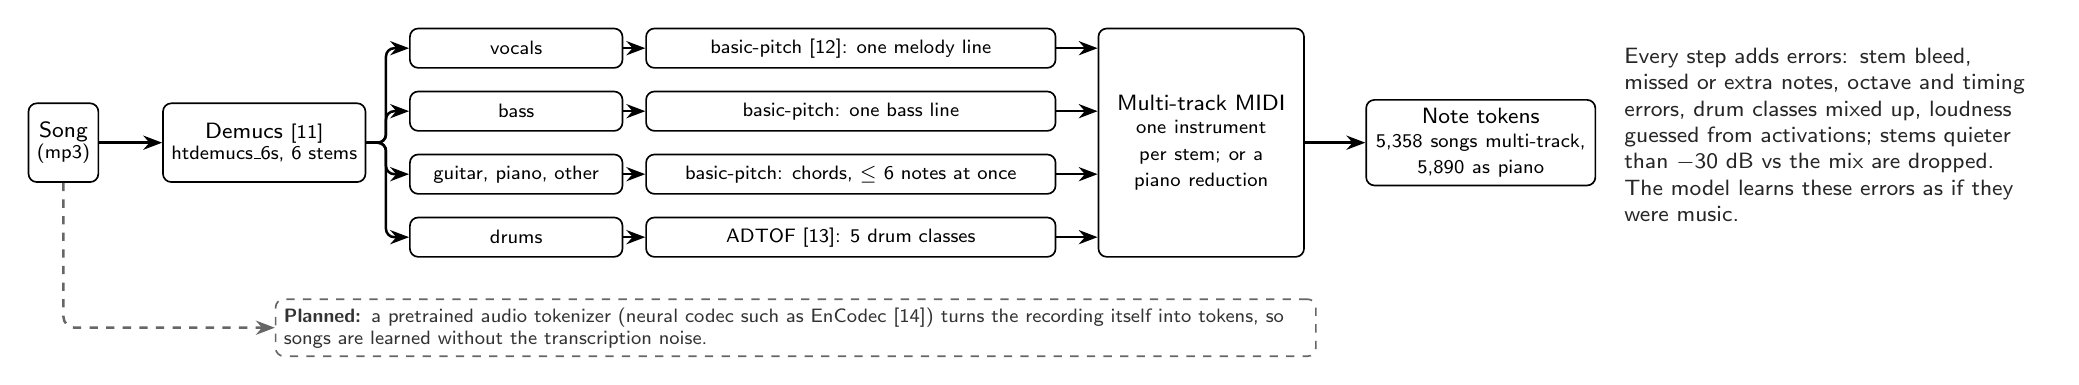
\begin{tikzpicture}
  \node[box, minimum height=10mm] (mp3) at (0, 0) {Song\\[-2pt] {\scriptsize (mp3)}};
  \node[box, minimum height=10mm] (dm) at (2.55, 0) {Demucs \rcite{11}\\[-2pt] {\scriptsize htdemucs\_6s, 6 stems}};
  \draw[arr] (mp3) -- (dm);
  \foreach \n/\t/\y [count=\i] in {vocals/{basic-pitch \rcite{12}: one melody line}/1.2, bass/{basic-pitch: one bass line}/0.4,
      {guitar, piano, other}/{basic-pitch: chords, $\le$ 6 notes at once}/-0.4, drums/{ADTOF \rcite{13}: 5 drum classes}/-1.2} {
    \node[box, minimum width=27mm, font=\scriptsize, minimum height=5mm] (st\i) at (5.75, \y) {\n};
    \node[box, minimum width=52mm, font=\scriptsize, minimum height=5mm] (tr\i) at (10.0, \y) {\t};
    \draw[arr, rounded corners=3pt] (dm.east) -- ++(0.25, 0) |- (st\i.west);
    \draw[arr] (st\i) -- (tr\i);
  }
  \node[box, minimum height=29mm, text width=24mm] (mid) at (14.45, 0) {Multi-track MIDI\\[-1pt] {\scriptsize one instrument per stem; or a piano reduction}};
  \foreach \i in {1,...,4} { \draw[arr] (tr\i.east) -- (mid.west |- tr\i.east); }
  \node[box, minimum height=10mm, text width=27mm] (tk) at (18.0, 0) {Note tokens\\[-1pt] {\scriptsize 5,358 songs multi-track, 5,890 as piano}};
  \draw[arr] (mid) -- (tk);
  \node[font=\scriptsize, text=black!85, align=left, anchor=west, text width=5.3cm, font=\footnotesize] at (19.7, 0.1) {Every step adds errors: stem bleed, missed or
    extra notes, octave and timing errors, drum classes mixed up, loudness guessed from activations; stems quieter than
    $-30$ dB vs the mix are dropped. The model learns these errors as if they were music.};
  \node[box, dashed, draw=black!60, text=black!80, font=\scriptsize, text width=13.0cm, align=left] (plan) at (9.3, -2.35)
    {\textbf{Planned:} a pretrained audio tokenizer (neural codec such as EnCodec \rcite{14}) turns the recording itself
     into tokens, so songs are learned without the transcription noise.};
  \draw[arr, dashed, black!60, rounded corners=4pt] (mp3.south) |- (plan.west);
\end{tikzpicture}}%

\newsavebox{\glossBox}
\sbox{\glossBox}{\scriptsize\renewcommand{\arraystretch}{1.2}%
\begin{tabular}{@{}>{\bfseries}l>{\raggedright}p{4.4cm}@{\hspace{12pt}}>{\bfseries}l>{\raggedright\arraybackslash}p{4.4cm}@{}}
CE & cross-entropy of the true notes (nats per note), the sum over the note's heads & D & distance to real music: weighted sum over takeover, top share, notes/s (0.20 each), out of band, instruments (0.15), runaway (0.10) of $|$system $-$ real$|$ / the real rows' spread\\
held-out captioned & 3,648 captioned GigaMIDI files kept out of training & runaway & continuation: share of rows above 40 notes per second; text and Q: share of 10-s windows above it\\
clean GigaMIDI & the base run's validation set (no captions) & takeover & one instrument plays over 80\% of a row's notes\\
caption gain & CE without the caption (or with a shuffled one) minus CE with it, on the same notes & out of band & share of new notes on instruments the prompt did not use\\
switch score & how far a section caption moves the music after a switch (section 3) & copies & share of new pitched notes inside verbatim copies of $\ge$ 16 chords\\
F & text follow score: mean over caption pairs (\capt{fast} vs \capt{slow}, ...) of the move in the asked direction over a clearly audible one (15 notes/s, 12 semitones, 8 velocity levels, 0.4 instrument share), clipped to $[-1, 1.5]$ & caption match & 0--1: mean over the categories a caption asks about (instruments, key, pace / loudness / register levels) of how well the piece meets them, half credit for near misses; 1 if nothing is checkable; judged with our caption builder's thresholds, so it favours our models\\
WSD \rcite{7} & warmup, stable, decay: LR schedule with a short final cooldown & J & F $- 0.25\,Q$; Q = D of the caption-free rows (no out-of-band term) + 4 $\times$ (runaway share over 0.10) + 4 $\times$ (copies over 0.25)\\
Muon \rcite{6} & optimizer that orthogonalises the update of each weight matrix & GQA \rcite{10} & grouped-query attention: groups of query heads share one key / value head\\
guidance \rcite{9} & classifier-free guidance: logits pushed away from the caption-free ones & stem & one separated part of a recording (vocals, bass, drums, ...)\\
\end{tabular}}%

\newsavebox{\refBox}
\sbox{\refBox}{\scriptsize\renewcommand{\arraystretch}{1.1}%
\newcommand{\rf}[3]{[#1] & #2, \href{https://arxiv.org/abs/#3}{\texttt{arXiv:#3}}\\}%
\newcommand{\rh}[3]{[#1] & #2, \href{https://huggingface.co/#3}{\texttt{hf.co/#3}}\\}%
\begin{tabular}{@{}r@{\hspace{4pt}}l@{}}
\rf{1}{The GigaMIDI Dataset (2025)}{2502.17726}
\rf{2}{Aria-MIDI: a dataset of piano MIDI files (2025)}{2504.15071}
\rh{3}{Discover MIDI Dataset}{datasets/projectlosangeles/Discover-MIDI-Dataset}
\rf{4}{MidiCaps: MIDI with text captions (2024)}{2406.02255}
\rf{5}{XMusic: the XMIDI dataset (2025)}{2501.08809}
\rf{6}{Muon is Scalable for LLM Training (2025)}{2502.16982}
\rf{7}{Scaling laws beyond fixed training durations: WSD (2024)}{2405.18392}
\rf{8}{MuseBarControl: counterfactual loss (2024)}{2407.04331}
\rf{9}{Classifier-Free Diffusion Guidance (2022)}{2207.12598}
\rf{10}{GQA: multi-query models from multi-head checkpoints (2023)}{2305.13245}
\rf{11}{Demucs: Hybrid Transformers for Music Source Separation (2022)}{2211.08553}
\rf{12}{basic-pitch: lightweight polyphonic note transcription (2022)}{2203.09893}
\rf{13}{ADTOF dataset (2021); the model used: Frame\_RNN, Zehren et al., Signals 2023}{2111.11737}
\rf{14}{EnCodec: High Fidelity Neural Audio Compression (2022)}{2210.13438}
\rf{15}{Anticipatory Music Transformer (2023)}{2306.08620}
\rh{16}{SkyTNT midi-model}{skytnt/midi-model-tv2o-medium}
\rh{17}{Music-Llama}{asigalov61/Music-Llama}
\rf{18}{MIDI-LLM (2025)}{2511.03942}
\rf{19}{Text2midi (2024)}{2412.16526}
\rf{20}{Aria (2025)}{2506.23869}
\rf{21}{Moonbeam (2025)}{2505.15559}
\rf{22}{CLaMP 3: Universal Music Information Retrieval (2025)}{2502.10362}
\end{tabular}}%

\begin{tikzpicture}
\coordinate (L) at (0, 0);
\coordinate (R) at (\panelW, 0);

%% ================= title =================
\node[font=\fontsize{20}{22}\selectfont\bfseries, text=tealT, anchor=north] (title) at ($(L)!0.5!(R)$) {What was found and tested};
\node[font=\footnotesize, text=black!85, anchor=north, align=center] (sub) at (title.south) {The evidence behind the
  captioned music model (477M; the model itself is on the first sheet, \textit{Captioned music model}): how it compares with
  other open MIDI models,\\ what F1 and its caption phase changed, and the pilots that chose each part.
  \textcolor{tealT}{\textbf{Teal}} = what the model uses / our models; \textcolor{altG}{\textbf{grey}} = the alternatives;
  \textcolor{pinkL}{pink} = captions.};

%% ================= 1: head-to-head =================
\coordinate (A) at ($(L |- sub.south)+(0, -1.1)$);
\node[cell, text width=8.6cm] (h1) at (A) {%
  {\footnotesize\bfseries Continuation: 32 prompts, 1,000 new notes each}\\[3pt]
  \usebox{\curveHH}\\[2pt]
  $\bullet$ the first 1,000 new notes, $\circ$ the first 200. On these 32 prompts both of our models continue closer to
  the real music on these density and instrument-use statistics than every other open model run here; 96 prompts do not
  keep that order (below). Over the first 200 every model is closer, SkyTNT medium passes musicar-L-caption (0.184 vs
  0.198) and musicar-L stays closest (0.090). D in units of the real rows' spread (with a floor); 0 = the real
  continuations.};
\node[cell, text width=16.4cm] (h2) at (h1.north east) {%
  {\footnotesize\bfseries The row metrics behind D (mean over the 32 rows)}\\[5pt]
  \usebox{\hhTable}\\[6pt]
  \textbf{Setup.} Every system writes MIDI for one frozen prompt set; every file is read back from the MIDI and scored the
  same way, per note and per second, never per token, so the tokenizers never enter. Prompts: the 32 clean GigaMIDI
  validation files of the sample evaluation (128 notes, $\ge$ 3 instruments, evenly spaced). Each model runs with its
  authors' sampling (AMT top-p 0.98; SkyTNT and Music-Llama $T$ 1.0, top-p 0.94, top-k 20; Moonbeam $T$ 0.9, top-p 0.95
  from its README and $T$ 0.6, top-p 0.9 from its completion example, its 1,024-position window restarted on the last
  768 notes by the harness, not the authors' scheme); ours with their presets
  (musicar-L $T$ 0.9; musicar-L-caption the app's f1 preset, no caption).\\[4pt]
  \textbf{Where the distance comes from.} musicar-L: its top instrument plays a little more (top share 0.418 vs
  0.390), it uses under one instrument fewer (6.9 vs 7.7) and it stays closer to the prompt's band (10\% vs 15\% out of
  band). musicar-L-caption: 0.14 of its 0.218 is density: it plays half as many notes per second (12.8 vs 24.0)
  and ends its piece inside the 1,000 notes in 53\% of the rows (length training: no length asked = a short piece).
  AMT: one instrument takes over 9\% of the rows. SkyTNT and Music-Llama: almost no new instruments (0--2\% out of band vs
  15\% in the real music), 5.3--5.7 instruments, and Music-Llama runs away in a quarter of the rows. Moonbeam plays twice the real density (49.5 notes per
  second: 0.33 of its 0.703), runs away in 31\% of the rows and lets one instrument take over 16\%; its density climbs
  inside the first window, before any restart (rows over 40 notes per second: 16\% of its first 200 new notes, 46\% of
  notes 447--894; real 13\% and 18\%). At $T$ 0.6 its density stays flat except in 2 files that stack notes on one
  onset (most of its 85.9 notes per second), and it copies more (46\%). Verbatim copies:
  musicar-L 14\%, SkyTNT 14\%, musicar-L-caption 0 (DRY).};
\path let \p1 = (h1.south), \p2 = (h2.south), \n1 = {min(\y1, \y2)} in coordinate (A2) at (0, \n1);
\node[cell, text width=8.6cm] (h3) at (A2) {%
  {\footnotesize\bfseries Piano: 32 prompts, 1,000 new notes each}\\[3pt]
  \usebox{\curveHHp}\\[2pt]
  $\bullet$ the first 1,000 new notes, $\circ$ the first 200. Solo-piano prompts from our held-out split of Aria-MIDI
  (Aria may have seen these files in training). For solo piano D reduces to notes per second and runaway.};
\node[cell, text width=16.4cm] (h4) at (h3.north east) {%
  {\footnotesize\bfseries The row metrics behind D (mean over the 32 rows)}\\[5pt]
  \usebox{\hhPiano}\\[6pt]
  Aria runs with its authors' CUDA sampler at the README's settings ($T$ 0.98, min-p 0.035), ours at $T$ 0.9. Both
  continuation models of ours are closer to the real note rate than Aria: it plays faster (10.0 vs 8.0 notes per second)
  and runs away in 1 row of 32. The 450M piano-cover fine-tune is the one model of ours behind Aria: trained to
  write covers that end, it plays 3.5 notes per second and ends every row inside the 1,000 notes.};
\path let \p1 = (h3.south), \p2 = (h4.south), \n1 = {min(\y1, \y2)} in coordinate (A3n) at (0, \n1);
\node[cell, text width=8.6cm] (h3n) at (A3n) {%
  {\footnotesize\bfseries Continuation and piano on 96 prompts (2026-10-31)}\\[3pt]
  \usebox{\curveHHn}\\[2pt]
  $\bullet$ the first 1,000 new notes, $\circ$ the first 200, all 96 prompts: the published 32 + 64 new ones. AMT, musicar-L
  and musicar-L-caption sit too close together to rank; musicar-L stays ahead of SkyTNT and Music-Llama. Moonbeam was not
  run on the 96.};
\node[cell, text width=16.4cm] (h4n) at (h3n.north east) {%
  {\footnotesize\bfseries D by prompt set: the published ranking does not hold; each row against its own real continuations (bold = lowest)}\\[5pt]
  \usebox{\hhGroups}\\[6pt]
  The published 32 all came from GigaMIDI's no-drums folder, so the 64 new prompts are 33 from it and 31 from the with-drums
  folder, the folders' share of the eligible files. D is a gap between means, so a system's errors can cancel over a wider
  set: AMT's 0.097 is below both its 0.289 and its 0.224. Paired bootstrap over prompts: musicar-L is closer than AMT in 26\%
  of the draws (59\% at 200 notes) and closer than SkyTNT medium and Music-Llama in all of them, at both lengths;
  musicar-L-caption is closer than AMT in 6\%, SkyTNT medium in 93\% (24\% at 200) and Music-Llama in 100\% (54\% at 200).
  The share of draws is no p-value. musicar-L-caption's gap is density again: 24 notes per second over the first 200 new notes,
  16.4 over 1,000 (real 24.5). AMT keeps the prompt's instruments least, which D does not score (0.77 vs real 0.92, musicar-L 0.89).\\[5pt]
  \usebox{\hhPianoN}\\[3pt]
  Piano: the order of the 32 prompts holds on 96, at both lengths. The percentages are draws closer than Aria at 1,000 notes.};
\path let \p1 = (h3n.south), \p2 = (h4n.south), \n1 = {min(\y1, \y2)} in coordinate (A3) at (0, \n1);
\node[cell, text width=8.6cm] (h5) at (A3) {%
  {\footnotesize\bfseries Text to MIDI: 27 captions + no caption, 16 pieces each, from the first note}\\[3pt]
  \usebox{\curveHHt}\\[2pt]
  \textcolor{black!85}{$\bullet$} English pairs, \textcolor{black!85}{$\circ$} Ukrainian pairs. On these short prompts
  every caption path of ours follows the captions better than both other open text-to-MIDI models, in both languages; on
  MidiCaps' long captions it is the other way round (below).};
\node[cell, text width=16.4cm] (h6) at (h5.north east) {%
  {\footnotesize\bfseries The scores behind F (mean over the 448 pieces of each system; 447 for MIDI-LLM and the band fine-tune: one file did not decode)}\\[5pt]
  \usebox{\textTable}\\[6pt]
  F over 9 English and 8 Ukrainian contrasts: \capt{fast} / \capt{slow}, \capt{minor} / \capt{major},
  \capt{loud} / \capt{soft}, \capt{high} / \capt{low} as caption pairs; \capt{solo piano}, \capt{a drum beat},
  \capt{without drums}, \capt{string ensemble}, \capt{electric guitar} each against no caption (no guitar prompt in
  Ukrainian). Caption match: see the glossary. Each model at its authors' sampling (MIDI-LLM $T$ 1.0, top-p 0.98;
  Text2midi $T$ 1.0); musicar-L-caption with the app's f1 preset and a 60-s length; with \texttt{-{}-retrieve} the caption also
  picks a real 128-note GigaMIDI opening that it continues (not in the file, hence 49 s; for the empty prompt a random
  opening of the same files). s50 and the band fine-tune of musicar-L (multi\_control: no text input, the caption
  picks the opening) keep the best of 4 candidates by caption match, so their rows are not single-sample scores. The 471M LaBSE encoder (frozen) is not counted in our
  parameters, Text2midi's FLAN-T5 encoder is.\\[4pt]
  \textbf{Ukrainian.} MIDI-LLM and Text2midi hardly move for Ukrainian captions (F 0.09 and 0.06): both learned text to
  MIDI from MidiCaps' English captions (MIDI-LLM: one Llama 3.2 1B with MIDI tokens added; Text2midi: FLAN-T5 +
  a decoder). musicar-L-caption reads both languages through LaBSE (F 0.95). They also run away more often (14\% and 9\%
  of 10-s windows over 40 notes per second vs 2\%) and their pieces are shorter (35 and 25 s: no length input, they stop at their authors' token budgets;
  musicar-L-caption, asked for 60 s: 64 s).};
\path let \p1 = (h5.south), \p2 = (h6.south), \n1 = {min(\y1, \y2)} in coordinate (Am) at (0, \n1);
\node[cell, text width=8.6cm] (h7) at (Am) {%
  {\footnotesize\bfseries MidiCaps test captions: 495 long English captions, one file each (2026-10-31)}\\[3pt]
  \usebox{\curveHHm}\\[2pt]
  \textcolor{tealT}{$\bullet$} musicar-L-caption, \textcolor{altG}{$\bullet$} MIDI-LLM, \textcolor{altG}{$\circ$} Text2midi;
  bars: the real files against another prompt's targets (floor) and against their own (ceiling). On captions it has not
  seen, musicar-L-caption is last on tempo, key, caption match and CLaMP 3, at the floor on tempo bins and key; on
  instruments it is level with Text2midi and behind MIDI-LLM.};
\node[cell, text width=16.4cm] (h8) at (h7.north east) {%
  {\footnotesize\bfseries The scores on the first 40 s (bold = best of the three models)}\\[5pt]
  \usebox{\hhMidicaps}\\[6pt]
  \textbf{Setup.} 500 captions from the 1,374 test rows of MidiCaps \rcite{4} that are outside GigaMIDI's train split, the replay
  store and any train file with the same notes; 5 of the 500 turned out to share notes with the replay store, so 495 are scored
  (Text2midi 492 usable files, the other 3 score 0). TB to CKD as in \rcite{19}, but tempo and key are estimated from the notes
  (our files carry no tempo event), which puts even the real files at 0.608 and 0.586, so compare these numbers only with each
  other and not with the papers'. MIDI-LLM $T$ 1.0, top-p 0.98, Text2midi $T$ 1.0, musicar-L-caption the app's f1 preset and 60 s.\\[4pt]
  \textbf{Reading.} Both other models learned text to MIDI from MidiCaps' captions, so this is their home ground as the
  short prompts are ours. CLaMP 3 agrees with each: on the short English prompts above its MRR is 0.321 for musicar-L-caption vs
  0.239 MIDI-LLM and 0.257 Text2midi, on MidiCaps 0.122 vs 0.276 and 0.156. The f1 preset was tuned on those short prompts, and
  never for key or tempo words inside long prose, so better settings may recover part of this; not tested yet.};
\path let \p1 = (h7.south), \p2 = (h8.south), \n1 = {min(\y1, \y2)} in coordinate (As) at (0, \n1);
\begin{scope}[on background layer]
  \draw[panel] (A) rectangle (R |- As);
\end{scope}
\node[ptitle] at (A) {\sect{1}{How it compares with other open MIDI models (head-to-head, 2026-10-29 to 31)}};

%% ================= 2: F1 =================
\coordinate (B) at ($(As)+(0, -1.1)$);
\node[cell, text width=8.1cm] (f1) at (B) {%
  {\footnotesize\bfseries F1: the caption run of the 450M (one RTX 5090)}\\[3pt]
  \usebox{\curveFone}\\[2pt]
  Every 1,000 steps (65,536 notes per step). \textcolor{tealT}{\textbf{Solid}}: held-out captioned GigaMIDI;
  \textcolor{tealB}{\textbf{dashed}}: the base's clean validation set. Off the scale at step 0: 2.181 / 2.109 (the start,
  f1\_plain512\_long, was trained at 512 notes). Window conditions off in these evals.};
\node[cell, text width=8.1cm] (f2) at (f1.north east) {%
  {\footnotesize\bfseries The caption phase: F1 $\to$ f1\_cap (600 steps at 512 notes)}\\[5pt]
  \usebox{\capTable}\\[6pt]
  In the pilots, the full recipe at 2,048 notes wore the caption reading down and a 512-note phase without
  spliced windows ($\approx$60 captioned openings per step vs 13.8) rebuilt it. On F1 the reading was intact and the
  phase leaves it flat. Cost: +0.016 CE at 2,048 notes. Gain: caption following at guidance 2 (+0.20 F) and the 120-s
  length. f1\_cap is musicar-L-caption.};
\node[cell, text width=8.1cm] (f3) at (f2.north east) {%
  {\footnotesize\bfseries Length control: 32 rows per length}\\[5pt]
  \usebox{\lenTable}\\[6pt]
  End / asked = median over the rows that end themselves; within 20\% = share of all rows. F1 and f1\_cap
  columns: $T$ 0.85, no top-p, no ramp; $^*$ EOS ramp 1, $T$ 1.1, top-p 0.9. Without a length the caption phase writes shorter pieces (66 vs 142 s). With the
  EOS ramp (+1 logit per second over) and the search's sampling, 120-s pieces land best (81\%); the ramp 0 / 0.5 runs at
  that sampling did not finish, so the ramp's own share is not measured. The app uses ramp 0.5 with a floor at 0.85 $L$
  and a stop at 1.2 $L$ (not measured as one set).};
\path let \p1 = (f1.south), \p2 = (f2.south), \p3 = (f3.south), \n1 = {min(\y1, \y2, \y3)} in coordinate (B2) at (0, \n1);
\node[cell, text width=12.4cm] (f4) at (B2) {%
  {\footnotesize\bfseries Decoding settings: a search on f1\_cap (2026-10-29)}\\[3pt]
  24 settings $\times$ 8 rows, then the best 8 $\times$ 16 rows, then 3 $\times$ 32 rows of 2,048 notes; score
  J = F $- 0.25\,Q$, settings with runaway $> 20\%$ or copies $> 25\%$ out. \textbf{Winner} (the app's f1 preset): guidance
  2.5, temperature 1.1, DRY on pitch-class chords (3, from 16 chords): F 1.07, F over the last notes 0.97, J 0.786. The
  defaults at 512 notes: J 0.34 and out (copies 0.48). Tested and not used: best of 4 / 8 (F 1.01 / 1.00 but D 2.13), a real
  opening picked by the caption (F 1.27 but copies 0.41), guidance against a neutral or the paired caption, guidance
  schedules, min-p. The F1 weights before the caption phase: J 0.30 with the best stage-A setting (f1\_cap 0.62).};
\node[cell, text width=11.9cm] (f5) at (f4.north east) {%
  {\footnotesize\bfseries Holding the style of the opening (generation only)}\\[3pt]
  Long pieces drifted: the density and the instruments changed every section even with one caption. Keep-style turns the
  first 256 notes' own description into the section caption of the rest; lock-instruments keeps their instruments
  (+ families the caption names that have not played yet). 3 captions $\times$ 2 seeds $\times$ 120 s: busiest / calmest
  quarter 8.1$\times$ $\to$ 4.3$\times$ in notes per second, loudness swing 16 $\to$ 7 levels, instruments in the last
  quarter 10 $\to$ 4. \capt{busy} / \capt{dense} are not held above 25 notes per second: held, they pushed 1 piece in 6
  into a runaway.};
\path let \p1 = (f4.south), \p2 = (f5.south), \n1 = {min(\y1, \y2)} in coordinate (Bs) at (0, \n1);
\begin{scope}[on background layer]
  \draw[panel] (B) rectangle (R |- Bs);
\end{scope}
\node[ptitle] at (B) {\sect{2}{F1 and the caption phase: captions, sections and length on the 450M (2026-10-27 / 28)}};

%% ================= 3: section recipe (107M pilots) =================
\coordinate (C) at ($(Bs)+(0, -1.1)$);
\node[cell, text width=11.4cm, font=\footnotesize] (s1) at (C) {%
Without these measures the model follows the first section's caption and then ignores later ones.\\[5pt]
\textbf{1. Change-aware captions.} Each section caption names what changed since the section before
(\capt{drums enter, louder}).\\[5pt]
\textbf{2. Spliced windows (50\% of windows).}\\[2pt]
\usebox{\spliceBox}\\[2pt]
File A up to a section boundary, then a section of file B (dashed) with B's caption and no file caption: the caption
contradicts the context and has to win.\\[5pt]
\textbf{3. Caption repeated every 64 notes,} in training and in generation.\\[2pt]
\usebox{\repeatBox}\\[5pt]
\textbf{4. Section words from section statistics.} Loudness, pace and register words use thresholds over sections, not
whole files (\capt{loud} = the loudest 20\% of sections), and pace is split into rhythm (onsets per second) and texture
(notes per onset), so a section caption does not push the music to extremes.\\[5pt]
\textbf{5. Caption dropout $\to$ guidance.} File captions are replaced by null vectors 15\% of the time, section
captions 20\%, so generation can use classifier-free guidance \rcite{9}.};
\node[cell, text width=7.4cm] (s2) at (s1.north east) {%
  {\footnotesize\bfseries Section-caption measures (107M pilot, 1,500--2,700 steps)}\\[3pt]
  \usebox{\curveArms}\\[2pt]
  Each row continues the same model (v2\_A0) for 1,500 steps with one measure or several; the last row runs 2,700 steps,
  the wall time of ``all three'' (no second forward). v2 words: measure 4. One seed, no error bars.
  \textcolor{tealT}{\textbf{Teal}} = the recipe in use.};
\node[cell, text width=5.6cm] (s3) at (s2.north east) {%
  {\footnotesize\bfseries Switch test}\\[3pt]
  6 prompt pairs A/B (e.g. soft / loud), 16 samples each; the section caption changes at note 1,024, guidance 2. The
  matching attribute (velocity, notes per second, register, drum or string share) is measured per 256 notes; the score
  is its change after the switch over its offset before it (0 = keeps the first style, 1 = a full flip). Start model:
  0.01.\\[4pt]
  {\footnotesize\bfseries Counterfactual loss \rcite{8}: not used}\\[3pt]
  The true caption must beat the previous one by 0.05 nats on the changed section's first 32 notes: alone 0.13, with
  splice and repeat 0.85, at 1.8$\times$ the step time.\\[4pt]
  {\footnotesize\bfseries At 450M (F1)}\\[3pt]
  Section captions beat shuffled ones by +0.004 (F1) / +0.006 (f1\_cap) nats per note on held-out files; no switch test
  on F1 / f1\_cap yet (the 450M rehearsal with the GQA merge showed no switch at guidance 2). Holding a caption still overshoots at 107M: asked for strings, 34\% of samples run away.};
\path let \p1 = (s1.south), \p2 = (s2.south), \p3 = (s3.south), \n1 = {min(\y1, \y2, \y3)} in coordinate (Cs) at (0, \n1);
\begin{scope}[on background layer]
  \draw[panel] (C) rectangle (R |- Cs);
\end{scope}
\node[ptitle] at (C) {\sect{3}{Section captions: what makes a later caption win (107M pilots)}};

%% ================= 4: why these choices =================
\coordinate (D) at ($(Cs)+(0, -1.1)$);
\node[cell, text width=8.1cm] (c1) at (D) {%
  {\footnotesize\bfseries Trunk block (42M, 98M notes, 3 seeds each)}\\[3pt]
  \usebox{\curveBlock}\\[2pt]
  Clean GigaMIDI validation. \textcolor{tealT}{\textbf{New}}: RMSNorm, SwiGLU, QK-norm; \textcolor{altG}{\textbf{old}} (dashed):
  LayerNorm, GELU; both RoPE and Muon. Thin lines = seeds, thick = mean; $-0.75$ at the end.};
\node[cell, text width=8.1cm] (c2) at (c1.north east) {%
  {\footnotesize\bfseries Base model pretraining (464M, 8.3B notes): musicar-L}\\[3pt]
  \usebox{\curveBase}\\[2pt]
  Clean GigaMIDI validation every 2,000 steps (65,536 notes per step); constant LR, then the $1-\sqrt{\cdot}$ cooldown in the
  last 20\%. One run on one RTX 5090, $\approx$41 h.};
\node[cell, text width=8.1cm] (c3) at (c2.north east) {%
  {\footnotesize\bfseries Output heads (42M, 98M notes)}\\[3pt]
  \usebox{\curveHeads}\\[2pt]
  Held-out GigaMIDI. \textcolor{tealT}{\textbf{Cascade}}: each head reads the values already chosen, 3 seeds (thin) and
  mean. \textcolor{altG}{\textbf{No chain}} (dashed): the same residual heads, each reading $h_t$ alone;
  \textcolor{altG}{\textbf{linear}} (dotted): one linear layer per attribute; one seed each.};
\path let \p1 = (c1.south), \p2 = (c2.south), \p3 = (c3.south), \n1 = {min(\y1, \y2, \y3)} in coordinate (D2) at (0, \n1);
\node[cell, text width=9.9cm] (c4) at (D2) {%
  {\footnotesize\bfseries GQA conversion (107M pilot, 12 $\to$ 4 key / value heads)}\\[3pt]
  \usebox{\curveGQA}\\[2pt]
  v2\_A0 converted, then 1,500 steps on the section recipe's data, LR $10^{-4}$, no section measures; the
  \textcolor{tealT}{\textbf{teal}} line is the same 1,500 steps without the conversion (full attention, what F1 uses).
  Off the scale at the start: mean-pool 10.15, merge 3.86--3.88. One seed.};
\node[cell, text width=14.9cm] (c5) at (c4.north east) {%
  {\footnotesize\bfseries GQA \rcite{10}: how a trained model is converted, and why F1 does not use it}\\[4pt]
  \textbf{What it buys.} Each group of 3 query heads shares one key / value head: the K / V projections and the KV cache
  shrink 3$\times$, so the 450M has 49.5M fewer parameters (464M $\to$ 415M without the caption adapters). Generation
  reads less per note: the 107M decodes 1.03$\times$ faster at 1 row and 2.28$\times$ at 64 rows (laptop GPU, bf16); on the
  Raspberry Pi (int4 weights, int8 cache) the estimate from bytes read per note is $\approx$1.3$\times$ at 1 row and
  $\approx$2.1$\times$ for 4 candidates with guidance.\\[4pt]
  \textbf{Merge.} Mean-pooling a group's K / V weights starts at CE 10.15. Instead, each group's value heads are merged
  by a PCA of their outputs weighted by the output projection, and the key heads per RoPE rotation pair by a rank-1
  complex merge weighted by the query energy, so RoPE stays exact. Measured on 16 batches of the model's own inputs.\\[4pt]
  \textbf{Transfer.} 300 steps in which only the attention layers train, each to reproduce its own full-attention output
  (relative MSE) on the original layer inputs, LR $10^{-3}$; the rest of the model is frozen.\\[4pt]
  \textbf{Result at 107M.} After 1,500 steps: mean-pool $+0.200$ vs full attention, merge only $+0.069$, merge +
  transfer $+0.040$ and still closing.\\[4pt]
  \textbf{At 450M it failed.} The 450M has QK-norm (the 107M pilots do not), and the merge flattened its attention:
  held-out CE 2.01 $\to$ 6.57 at the merge. An F1 rehearsal with the merge ended at 2.115 after 2,400 steps; the same
  recipe with full attention reached 2.058 in 600. GQA was not what kept the 450M from reading captions either.
  So F1 kept full attention; a conversion for the Raspberry Pi, if needed, is its own step (attention transfer first,
  CE within 0.05 of the captioned model before any further training).};
\path let \p1 = (c4.south), \p2 = (c5.south), \n1 = {min(\y1, \y2)} in coordinate (D3) at (0, \n1);
\node[cell, text width=9.2cm] (c6) at (D3) {%
  {\footnotesize\bfseries Per head at step 1,500 (seed 1337, nats / note)}\\[5pt]
  {\renewcommand{\arraystretch}{1.3}\setlength{\tabcolsep}{5pt}%
  \begin{tabular}{@{}lrrrrrr@{}}
  heads & $\Delta t$ & pitch & dur. & vel. & sum & instr.\\\hline
  \textcolor{tealT}{\textbf{cascade}} & 0.285 & 0.779 & 0.966 & 0.737 & \textbf{2.766} & 0.315\\
  no chain & 0.281 & 0.956 & 1.025 & 0.844 & 3.106 & 0.346\\
  linear & 0.286 & 0.970 & 1.037 & 0.853 & 3.145 & 0.353\\
  \end{tabular}}};
\node[cell, text width=15.6cm] (c7) at (c6.north east) {%
  {\footnotesize\bfseries What the chain buys}\\[3pt]
  The chain is worth $-0.34$ nats per note at the end (pitch $+0.18$, velocity $+0.11$ without it), the residual head
  form only $-0.04$. $\Delta t$ is the first head, so it reads nothing extra and is the same in all three. Pitch gains
  most from the chain ($-0.18$): knowing when the note starts and on which instrument narrows its pitch. The sum is the
  held-out CE above; the instrument head is reported apart. An earlier 6M piano A/B (4 heads, chained plain MLP heads)
  had found only $-0.03$ for the chain: there its pitch head had lost the direct path from $h_t$.};
\path let \p1 = (c6.south), \p2 = (c7.south), \n1 = {min(\y1, \y2)} in coordinate (Ds) at (0, \n1);
\begin{scope}[on background layer]
  \draw[panel] (D) rectangle (R |- Ds);
\end{scope}
\node[ptitle] at (D) {\sect{4}{Why these choices: training curves (teal = what the model uses)}};

%% ================= 5: training stages =================
\coordinate (E) at ($(Ds)+(0, -1.1)$);
\begin{scope}
  \clip[rounded corners=8pt] (E) rectangle ++(\wd\setupBox, -\ht\setupBox-\dp\setupBox);
  \node[anchor=north west, inner sep=0pt] (setup) at (E) {\usebox{\setupBox}};
\end{scope}
\draw[rounded corners=8pt, draw=greyB, line width=1pt] (setup.south west) rectangle (setup.north east);
\node[ptitle] at (setup.north west) {\sect{5}{Training stages}};

%% ================= 6: audio -> MIDI =================
\node[anchor=north west, inner sep=10pt] (audio) at ($(setup.south west)+(0, -1.1)$) {\usebox{\audioBox}};
\begin{scope}[on background layer]
  \draw[panel] (audio.south west) rectangle (audio.north east -| R);
\end{scope}
\node[ptitle] at (audio.north west) {\sect{6}{Audio $\to$ MIDI: how songs become training notes (fine-tune data)}};

%% ================= 7: glossary, 8: references (same height) =================
\node[anchor=north west, inner sep=10pt] (gloss) at ($(audio.south west)+(0, -1.1)$) {\usebox{\glossBox}};
\node[anchor=north east, inner sep=10pt] (refs) at (gloss.north -| R) {\usebox{\refBox}};
\begin{scope}[on background layer]
  \path let \p1 = (gloss.south), \p2 = (refs.south), \n1 = {min(\y1, \y2)} in
    [panel] (gloss.north west) rectangle ([xshift=-0.6cm]refs.west |- 0, \n1)
    [panel] (refs.north west) rectangle (refs.east |- 0, \n1);
\end{scope}
\node[ptitle] at (gloss.north west) {\sect{7}{Glossary}};
\node[ptitle] at (refs.north west) {\sect{8}{References (links)}};

\end{tikzpicture}
\end{document}
